\documentclass[border=5pt]{standalone}
\usepackage{fontspec,xeCJK,amsmath,amssymb,tikz,graphicx}
\usetikzlibrary{arrows.meta,calc}
\setmainfont{Arial}\setCJKmainfont{PingFang SC}
\definecolor{ink}{HTML}{203340}\definecolor{blue}{HTML}{147E91}\definecolor{pale}{HTML}{EEF6F6}\definecolor{warm}{HTML}{AD651E}\definecolor{cream}{HTML}{FFF6E9}\definecolor{line}{HTML}{CFDDDF}
% Cropped imagegen illustrations retained; exact notation and computation added in TeX.
\newcommand{\strip}[2]{\begin{scope}\clip(.65,#1)rectangle(10.35,#1+2.3);\node[anchor=north west,inner sep=0]at(.65,#1+2.3+#2){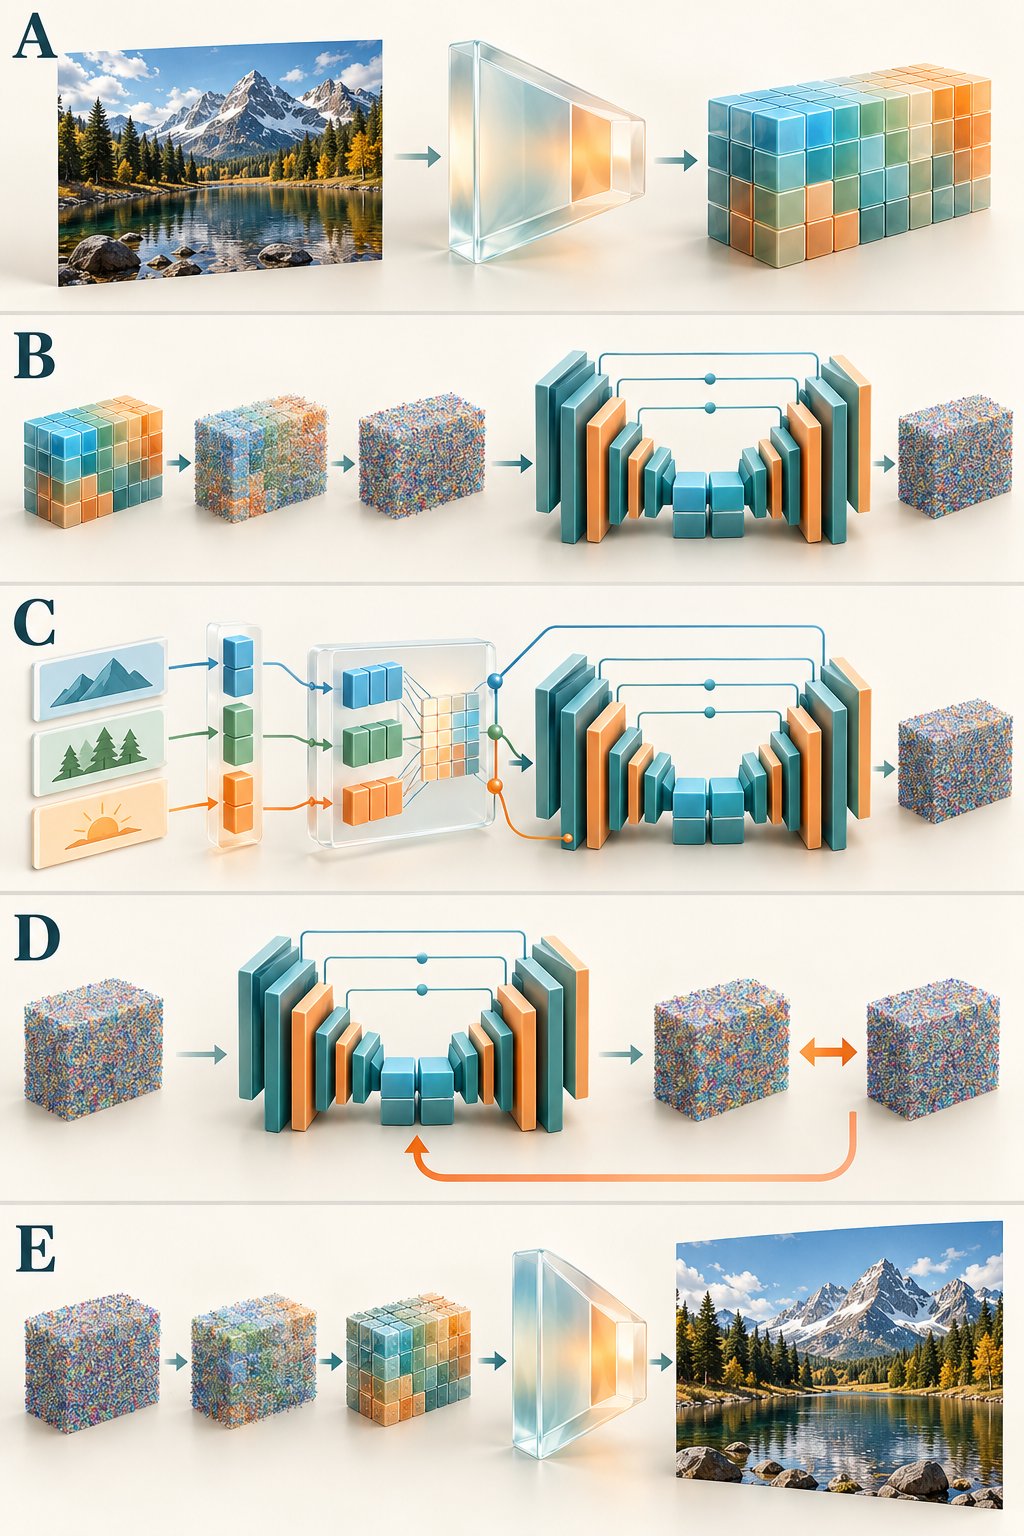
\includegraphics[width=9.7cm]{ldm-imagegen-draft.png}};\fill[white](.65,#1+1.85)rectangle(1.4,#1+2.3);\end{scope}}
\begin{document}
\begin{tikzpicture}[x=1cm,y=1cm,every node/.style={text=ink,font=\fontsize{11}{14}\selectfont},flow/.style={-{Stealth[length=5pt]},draw=blue,line width=1pt},box/.style={rounded corners=5pt,draw=line,fill=white}]
\path[use as bounding box](0,0)rectangle(11,31.8);\fill[pale](0,0)rectangle(11,31.8);
\node[font=\fontsize{21}{25}\selectfont\bfseries]at(5.5,31.05){LDM：把去噪搬进小空间};
\node[text=blue]at(5.5,30.35){先学压缩器　再学潜空间生成　最后解码成图};
\draw[box](.3,24.9)rectangle(10.7,29.8);
\node[anchor=west,font=\fontsize{14}{17}\selectfont\bfseries]at(.6,29.25){A　感知压缩｜原文 §3.1};
\strip{26.55}{.42}
\node at(5.5,26.05){$x\ (H\times W\times3)\ \xrightarrow{\mathcal E}\ z\ (h\times w\times c)$};
\node[font=\fontsize{10}{13}\selectfont]at(5.5,25.45){重建 $\mathcal D(\mathcal E(x))$；感知 + 对抗 + 弱正则；阶段一训练};
\draw[box](.3,19.5)rectangle(10.7,24.5);
\node[anchor=west,font=\fontsize{14}{17}\selectfont\bfseries]at(.6,23.95){B　造一道去噪题｜原文 §3.2};
\strip{21.25}{3.30}
\node at(5.5,20.75){$z_t=\sqrt{\bar\alpha_t}z_0+\sqrt{1-\bar\alpha_t}\epsilon$};
\node[font=\fontsize{10}{13}\selectfont]at(5.5,20.05){抽一个 $t$；U-Net 接收 $z_t,t$，输出同形状噪声 $\hat\epsilon$};
\draw[box](.3,13.8)rectangle(10.7,19.1);
\node[anchor=west,font=\fontsize{14}{17}\selectfont\bfseries]at(.6,18.55){C　让条件参与｜原文 §3.3};
\strip{15.65}{5.86}
\node at(5.5,15.1){条件 $y\to\tau_\theta(y)$；$Q\gets$图像特征，$K,V\gets$条件};
\node at(5.5,14.45){$\operatorname{softmax}(QK^\top/\sqrt d)V$；空间条件也可拼接};
\draw[box,fill=cream](.3,8.1)rectangle(10.7,13.4);
\node[anchor=west,font=\fontsize{14}{17}\selectfont\bfseries]at(.6,12.85){D　阶段二训练｜固定 $\mathcal E,\mathcal D$};
\strip{9.95}{8.87}
\node at(5.5,9.4){$L=\mathbb E\lVert\epsilon-\epsilon_\theta(z_t,t,\tau_\theta(y))\rVert^2$};
\node[font=\fontsize{10}{13}\selectfont,text=warm]at(5.5,8.75){真实噪声对照预测；更新去噪网络与条件编码器};
\draw[box](.3,2.35)rectangle(10.7,7.7);
\node[anchor=west,font=\fontsize{14}{17}\selectfont\bfseries]at(.6,7.15){E　生成与检验｜原文 §4--6};
\strip{4.3}{11.71}
\node at(5.5,3.7){$z_T\sim\mathcal N(0,I)\to\cdots\to z_0\xrightarrow{\mathcal D}\hat x$};
\node[font=\fontsize{10}{13}\selectfont]at(5.5,3.0){参数固定；反复调用 B/C 去噪；标准生成最后解码一次};
\node[font=\fontsize{10}{13}\selectfont,text=blue]at(5.5,1.6){训练路线：A 预训练后冻结，B + C $\to$ D};
\node[font=\fontsize{10}{13}\selectfont,text=blue]at(5.5,.95){运行路线：E 从噪声出发；§4 比较倍率、速度和条件任务};
\node[font=\fontsize{9}{12}\selectfont]at(5.5,.35){全文：§1--2 为什么搬；§3 A/B/C/D 怎么搬；§4--6 E 搬得值不值};
\end{tikzpicture}\end{document}
